% DSA5208 Project 3 report (English version; the Chinese version is main_zh.tex
% and follows the same structure). Sections marked \todo{} are filled in as the
% corresponding parts are built and measured.
\documentclass[11pt,a4paper]{article}

\usepackage[margin=2.3cm]{geometry}
\usepackage{amsmath,amssymb}
\usepackage{booktabs}
\usepackage{graphicx}
\usepackage{xcolor}
\usepackage{listings}
\usepackage{hyperref}
\usepackage{enumitem}

\newcommand{\todo}[1]{\textcolor{red}{[TODO: #1]}}
\newcommand{\code}[1]{\texttt{#1}}

\lstset{basicstyle=\ttfamily\small, columns=fullflexible, frame=single, breaklines=true}

\title{Distributed Acceleration of Hierarchical PCA-QD Genetic-Programming Factor Mining\\[4pt]
\large DSA5208 Project 3}
\author{\todo{Name (Student ID)} \and \todo{Name (Student ID)} \and \todo{Name (Student ID)}}
\date{\todo{date}}

\begin{document}
\maketitle

\begin{abstract}
We accelerate an existing genetic-programming (GP) factor miner for Chinese A-share stocks. The search loop stays in Python; its batch evaluation engine is re-implemented in C++ and parallelised with MPI + OpenMP (factor computation and evaluation) and with CUDA (PCA signatures and similarity). The data are decomposed by trading date, which turns per-expression parallelism into a genuinely distributed computation: rolling operators need halo exchange or redundant computation, the exponential moving average needs a scan across ranks, and daily statistics need a global reduction. Shared subexpressions of a batch are merged into a DAG, so each is computed once.
\todo{headline numbers: speed-up and efficiency at 288 cores, GPU speed-up}
\end{abstract}

%======================================================================
\section*{Terminology}
\todo{one line each; every term below is used in the report}

\begin{tabular}{@{}ll@{}}
\toprule
Term & Meaning \\
\midrule
factor & a formula mapping raw stock data to a daily score per stock \\
panel & a $T\times N$ array (trading days $\times$ stocks) \\
RankIC & daily Spearman correlation between a factor and future returns \\
fitness & the GP objective computed from the RankIC (Section~\ref{sec:fitness}) \\
gene pool & the best expressions of a stage, reused as subtrees by deeper stages \\
PCA-QD signature & a short vector summarising a factor, used to measure similarity \\
DAG & directed acyclic graph of the distinct subexpressions of a batch \\
root & the DAG node of a whole expression (a candidate factor) \\
halo & history rows a rank needs from the ranks to its left \\
$H_0$ & redundant-computation budget (days of history recomputed locally) \\
ema & exponential moving average \\
strong / weak scaling & fixed total problem / fixed problem per rank \\
Karp--Flatt metric & experimentally determined serial fraction \\
\todo{more} & \\
\bottomrule
\end{tabular}

%======================================================================
\section{Background and algorithm}

\subsection{Factors and RankIC}
Every raw field is a panel $X\in\mathbb{R}^{T\times N}$ (days $\times$ stocks). A factor $F$ is computed from raw panels by an expression tree, for example $\mathrm{mean}(\text{volume}/\text{amount}, 10)$. A factor is useful if, on each day, the ranking of stocks by the factor predicts the ranking of their future returns $Y$. Its quality on day $t$ is
\begin{equation}
  \mathrm{IC}_t = \operatorname{corr}\!\big(\operatorname{rank}(F_{t,\cdot}),\ \operatorname{rank}(Y_{t,\cdot})\big),
  \qquad \overline{\mathrm{IC}} = \frac{1}{|T_{\mathrm{valid}}|}\sum_{t} \mathrm{IC}_t .
\end{equation}

\subsection{Expressions and operators}
Leaves are raw fields. Window lengths are taken from $\{1,5,10,15,20,30,60\}$. There are 20 operators:
\begin{itemize}[nosep]
  \item element-wise: $+,-,\times,\div,\log,|\cdot|$;
  \item cross-sectional: rank, z-score;
  \item rolling: mean, std, sum, max, min, median, ema, lag, delta, pct\_change;
  \item pairwise rolling: correlation, beta.
\end{itemize}
Expressions are normalised: commutative operands are ordered, $\mathrm{rank}(\mathrm{rank}(x))=\mathrm{rank}(x)$, and $x-x$, $x/x$ are rejected. Trees have at most 11 nodes.
\todo{size of the search space by depth}

\subsection{Fitness}
\label{sec:fitness}
A candidate must have a valid IC on at least $80\%$ of days and at most $20\%$ missing values. Let $m_1,\dots,m_4$ be the mean IC on four consecutive time segments. Then
\begin{equation}
  \text{fitness} = |\overline{\mathrm{IC}}| - 0.5\,\operatorname{std}(m_1,\dots,m_4) - 0.0005\max(\text{nodes}-3,0),
\end{equation}
and the fitness is multiplied by $0.25$ if fewer than $75\%$ of the segments share the sign of $\overline{\mathrm{IC}}$.

\subsection{Layer-wise generation}
Evolution runs in three stages, with maximum tree depth $1$, $2$ and $3$. Each stage evolves a population of $10{,}000$ for $10$ generations:
\begin{itemize}[nosep]
  \item parents are drawn from a feature-capped pool, by tournament or by $\varepsilon$-lexicase selection over the four IC segments;
  \item offspring come from same-level crossover and from feature, operator, window and subtree mutation; each family keeps its two best members;
  \item random immigrants make up $10\%$ of each generation;
  \item at the end of a stage, the best $2{,}000$ admitted expressions become a \emph{gene pool}; deeper stages build $70\%$ of their subtrees from these gene pools.
\end{itemize}

\subsection{PCA-QD diversity archive}
Many candidates are near-duplicates of each other. Comparing full factor panels pairwise costs $O(TN)$ per pair, which is prohibitive for thousands of candidates against thousands of archived factors. Each candidate is therefore compressed into a short signature:
\begin{enumerate}[nosep]
  \item take every 5th day and its cross-sectional percentile ranks (missing values set to $0.5$), and centre each row, giving $R\in\mathbb{R}^{T_s\times N}$;
  \item run four power iterations for the leading right singular vector $v$;
  \item set $s = Rv/\|Rv\|$, with its sign fixed.
\end{enumerate}
A candidate enters the archive if its $|$correlation$|$ with every archived signature is below $0.9$. Otherwise it replaces its nearest neighbour, but only if its RankIC is better by at least $0.002$. Admission is sequential.

\subsection{Cost of each part}
\label{sec:cost}
\todo{per expression: operators $O(TN)$ per node (median $O(TNw)$); RankIC $O(TN\log N)$; signature $O(T_s N k)$ for $k$ iterations; similarity $O(C\,A\,T_s)$ for $C$ candidates and $A$ archived signatures. These are the slopes compared with measurements in Section~\ref{sec:x1}.}

\subsection{The original implementation and its bottlenecks}
The Python engine evaluates each expression independently in a pool of 32 processes:
\begin{itemize}[nosep]
  \item shared subtrees are recomputed from raw data every time, because its cache stores only final scores;
  \item every process holds the full data, and parallelism is limited to the number of expressions in a batch;
  \item the signature is computed in single-threaded NumPy, and only the final similarity matrix multiplication uses the GPU.
\end{itemize}
A previous run selected $1481$ factors, with mean out-of-sample $|\mathrm{RankIC}|$ of $0.080$ in 2022.

%======================================================================
\section{Data}

\subsection{Real data}
The raw data are daily panels of 132 numeric fields for Chinese A-shares; part of the fields are aggregated from minute-frequency data to daily frequency. The label is a forward-return panel, masked to tradable, non-ST stocks. The evolution period (2016--2021) has $T=1461$ trading days and $N=5876$ stocks. The number of stocks with data grows from 2636 at the start of 2016 to 4845 at the end of 2021. Panels are exported once to raw little-endian float32 files in date-major layout (element $t\cdot N+s$), about $34$\,MB per field and $4.3$\,GB in total. The export reuses the original cleaning code, so the C++ engine sees exactly the values the Python miner sees.
\todo{list of field groups}

\subsection{Synthetic data}
Weak scaling needs a problem that grows with the number of ranks: with 64 days per rank, 288 ranks need $18{,}432$ days, far more than the 1461 real days. Synthetic panels are generated on demand, so a rank produces only its own rows. Every cell depends only on (seed, field, global day, stock), so results do not depend on the number of ranks:
\begin{itemize}[nosep]
  \item each field is either log-normal, $\exp(\mu + 0.5z)$ with $\mu\in[-2,6]$ (like prices, volumes and amounts), or normal, $\sigma z$ with $\sigma\in[0.01,1]$ (like returns and flows), chosen by a hash of the field name;
  \item the label is $0.02z$;
  \item $z\sim N(0,1)$ is drawn independently per cell, and $2\%$ of cells are missing.
\end{itemize}
Unlike the real data, the number of stocks per day is constant, so synthetic runs have no load imbalance from a growing stock universe.

%======================================================================
\section{Computing platform: Vanda}
\todo{NUS Vanda cluster: CPU nodes with 2$\times$ Intel Xeon 8452Y (72 cores) and 512\,GB; GPU nodes with NVIDIA A40 (48\,GB); 100\,Gb Ethernet between nodes; PBS queues and limits (free queue 160 cores per job, project queue used for 288 cores); home and scratch file systems; OpenMPI 5.0.8 and GCC 14.3; how ranks and threads are placed and bound.}

%======================================================================
\section{Parallel design}

\setcounter{subsection}{-1}
\subsection{Overview, decomposition and data layout}
\todo{figure of the whole pipeline: Python GP loop $\to$ C++ engine (factor computation and evaluation on CPU with MPI + OpenMP; signatures and similarity on GPU) $\to$ sequential admission. MPI+X: X = OpenMP for factor evaluation, CUDA for the PCA part.}

Each of the $p$ ranks owns a contiguous block of about $T/p$ days for all $N$ stocks. With this choice:
\begin{itemize}[nosep]
  \item cross-sectional work (ranking, daily IC) is local;
  \item time-series operators need data from the preceding blocks;
  \item global statistics need reductions.
\end{itemize}
We decompose the data rather than the expressions. Each rank evaluates every node of the batch DAG (Section~\ref{sec:dag}) level by level, but only on its own dates, so communication involves only a few boundary rows, never whole panels. Splitting by stock instead would make every cross-sectional rank a global sort; splitting by expression, as the Python version does, makes every process hold all data.
A panel is stored as a contiguous float32 array in date-major order, together with the index \code{lo}$\le0$ of its first stored row; rows below 0 hold history that precedes the rank's own block.

\subsection{Factor computation and evaluation}

\subsubsection{Operator classes and their parallel axis}
\label{sec:operators}
\begin{itemize}[nosep]
  \item element-wise operators sweep the array once, split over days;
  \item cross-sectional operators (rank, z-score) process one day (one row) at a time, split over days with dynamic scheduling;
  \item rolling operators process one stock (one column) at a time with $O(T)$ sliding-window updates, split over stocks; each thread copies the column into its own scratch array, computes, and writes back.
\end{itemize}
\todo{strided column access and why it is acceptable on the CPU}

\subsubsection{Reproducing pandas exactly}
Small differences in floating-point rounding can change which windows look constant, and hence whether a correlation is finite, so we port the pandas~3.0.3 window kernels rather than textbook formulas.
\begin{itemize}[nosep]
  \item Rolling sums and means use Kahan summation with separate compensations for additions and removals. When the last $n_{obs}$ observations are identical, the repeated value is returned exactly.
  \item Rolling variance uses Welford's update and recomputes the window from scratch when cancellation is detected ($m_2^{\text{prev}}\cdot10^3\varepsilon > m_2$).
  \item Windows count only non-missing observations. The minimum count is 1 for mean, sum and median, and $\min(3,w)$ for std, max, min, correlation and beta.
  \item Correlation and covariance use pairwise-complete observations. Beta divides by the variance of $b$ alone.
  \item Infinite results of $+,-,\times,\div$, pct\_change and beta become missing values. pct\_change is computed in float32, as in pandas.
\end{itemize}
Max and min use monotone deques, and the median keeps the window sorted ($w\le60$).

\subsubsection{Halo exchange versus redundant computation}
\label{sec:halo}
A rolling operator on the first days of a block needs earlier values, which belong to the ranks on the left. We consider three strategies:
\begin{itemize}[nosep]
  \item \textbf{A, redundant computation:} each rank preloads $H_0$ extra days of raw data and recomputes subtrees on them, without communication;
  \item \textbf{B, halo exchange:} after each DAG level, each rank sends the rows its right-hand ranks need; all nodes of the level are packed into one message per partner (\code{MPI\_Isend}/\code{MPI\_Irecv}). When blocks are shorter than the halo, a rank receives from several ranks to its left (multi-hop halo);
  \item \textbf{Hybrid:} a subtree is recomputed if its cumulative lookback is at most $H_0$, and exchanged otherwise.
\end{itemize}
$H_0$ is therefore a single tuning knob: $H_0=0$ gives strategy B, and $H_0\ge \max h$ gives strategy A. The redundant work per rank grows like $H_0/(T/p)$, while the number of messages grows with $p$ when blocks get short, so the best $H_0$ depends on $p$ and on whether neighbours share a node.

\subsubsection{Recursive operator: ema}
\label{sec:ema}
The exponential moving average follows pandas' \code{adjust=False} recursion with missing values: the previous weight decays by $(1-\alpha)$ every day, so after $k$ missing days
\begin{equation}
  y_t = \frac{o\,y_{\text{prev}} + \alpha x_t}{o+\alpha}, \qquad o = (1-\alpha)^{k+1}.
\end{equation}
This is an affine function of $y_{\text{prev}}$, so a block of days maps its initial state through an affine map, and affine maps compose associatively. Each rank summarises its block per stock; the states are then passed along the ranks in a chain (rank $r$ receives the state at its first day from rank $r-1$), and each rank runs its block from the correct initial state.
\todo{cost of the chain: $p-1$ hops; an \code{MPI\_Exscan} would need $O(\log p)$ steps (future work)}

\subsubsection{Daily RankIC and fitness}
Daily RankIC is local to a rank, because a day's cross-section is never split. A root's RankIC is computed as soon as its DAG level is done, and the root's panel is then released like any other node. Each rank keeps only a small summary per root (segment sums and counts), and one \code{MPI\_Allreduce} of all summaries gives the fitness of the whole batch.

\subsubsection{Thread strategies and memory}
\todo{two strategies: (i) operator-level, nodes one after another and each operator split over days or stocks; (ii) node-level, the nodes of one level spread over the threads, each single-threaded. Development findings: first-touch page faults, buffer pool kept across batches, per-thread scratch arrays.}

\subsubsection{Communication and load model}
\todo{halo bytes and messages per level as a function of $p$; ema chain; one Allreduce; load imbalance from the growing stock universe}

\subsection{PCA signatures and similarity on the GPU}
\todo{batched sampled ranking; batched power iteration (distributed: $Rv$ is local, $R^\top u$ needs one Allreduce of a length-$N$ vector per iteration, batched over factors); tiled similarity GEMM vs cuBLAS; sequential admission as the serial fraction}

\subsection{Power iteration versus Lanczos}
\todo{convergence of both depends on the singular-value gap; cost per iteration (one product with $R$ and one with $R^\top$); storage of the Lanczos basis; is four power iterations accurate enough for the admission decision?}

\subsection{The subexpression DAG, memory and caching}
\label{sec:dag}
A batch of expressions is merged into one DAG by \emph{hash-consing}. Before a node is created, the key (operator, window, child ids) is looked up in a hash table. An existing node is reused, so a subexpression shared by several candidates is computed once. Normalisation is applied during construction:
\begin{itemize}[nosep]
  \item the children of commutative operators are ordered by id;
  \item a rank whose child is a rank returns the child;
  \item equal children of $-$ and $\div$ reject the whole expression, which is rolled back.
\end{itemize}
Children are always created before their parents, so the node array is already a topological order. Every rank builds the identical DAG, so node ids agree across ranks and halo messages need no descriptors.

For each node we record its \emph{cumulative lookback} $h(n) = \ell(n) + \max_{c} h(c)$, where $\ell = w-1$ for rolling windows and $\ell = k$ for lag, delta and pct\_change, and its \emph{halo rows} $\max_{\text{parents }q} \ell(q)$. Each node also counts its parents; when all parents are computed, its panel goes back to a buffer pool.

On the $1481$ selected factors, merging all expressions into one DAG reduces $11{,}413$ tree nodes to $4{,}052$ distinct nodes, including leaves.
\todo{memory as a red--blue pebble game (Lecture 12): fast memory = RAM or GPU memory, slow = recomputation or host memory; peak memory of a batch; chunking wide levels; caching across batches and generations}

%======================================================================
\section{Validation}
\label{sec:validation}
Validation shows that the C++ engine and its parallel versions compute the same results as the original Python miner and as the serial engine.

\paragraph{Parsing and DAG.} We test 1531 expressions: the 1481 selected factors plus crafted cases for every operator and normalisation rule. For every valid expression, the C++ engine reproduces the Python depth and node count, and two expressions share a DAG root exactly when Python gives them the same normalised key.

\paragraph{Operators.} We evaluate 88 expressions on a $120\times300$ sample of the real data with all 132 fields: every operator with windows 1, 5 and 20, several nested expressions, and 40 selected factors. The number of cases follows from this design (operator $\times$ window, plus nesting), not from a target count. Each result is compared with the pandas output element by element, using $|q-p|\le 10^{-4}|p| + 10^{-5}\,\mathrm{rms}(p)$ and an identical pattern of missing values.
\todo{88/88 pass; bit-identical share; the float32 intermediate issue and how it was resolved}

\paragraph{RankIC, fitness and signatures.} \todo{88/88 RankIC/fitness to $10^{-12}$; signatures 88/88 code-identical, end-to-end $1-$similarity $\le 6.9\times10^{-6}$ on the full data}

\paragraph{Distributed against serial.} The distributed engine must give the same candidate validity as the serial engine and fitness within $10^{-5}$. Panels are not required to be bit-identical: rolling sums and variances (Kahan and Welford) restart at every block boundary, so a cell can differ in the last bits, and a near-zero cell can differ by a large relative amount without changing any ranking. Results for up to 288 ranks and both thread strategies are in Section~\ref{sec:v}.

%======================================================================
\section{Experiments}
Every run is timed with \code{MPI\_Barrier} followed by \code{MPI\_Wtime}. Each phase (loading, operators, halo exchange, ema scan, RankIC, waiting, reduction) is the maximum over ranks, and the total is the slowest rank's wall time. Each configuration runs once to warm up (which also fills the buffer pool, as in a GP run where the engine is called generation after generation) and then three times; we report the median. Unless stated otherwise the batch has 200 selected factors (752 DAG nodes) on the full real data, $T=1461$ days and $N=5876$ stocks. Loading is reported separately because it depends on the shared file system. All plots use logarithmic axes for time, problem size and core count. Runs used Intel Xeon 8452Y nodes only; each job records the CPU model of its hosts.

\subsection{Factor computation and evaluation}

\subsubsection{Serial run time against problem size}
\label{sec:x1}
One rank and one thread. We vary one dimension at a time: the number of days $T$ (prefixes of the real data, 50 factors), the number of stocks $N$ (the first $N$ stocks), and the batch size; synthetic data extend $T$ and $N$ beyond the real data (Figure~\ref{fig:x1}).

\begin{table}[h]
\centering
\begin{tabular}{lrrr}
\toprule
dimension & range & total time (s) & slope \\
\midrule
$T$, real, 50 factors & 91 -- 1461 & 2.34 -- 34.2 & 0.99 \\
$N$, real, 50 factors & 367 -- 5876 & 2.82 -- 34.1 & 0.93 \\
$T$, synthetic & 1461 -- 11688 & 64.9 -- 610.7 & 1.10 \\
$N$, synthetic & 5876 -- 23504 & 64.8 -- 273.1 & 1.05 \\
batch size, real & 25 -- 800 & 17.1 -- 525.2 & 0.99 \\
\bottomrule
\end{tabular}
\caption{Serial run time. The slope is fitted on log--log axes to the time without loading.}
\end{table}

The run time is close to linear in every dimension, as Section~\ref{sec:cost} predicts: operators are $O(TN)$ per node and RankIC is $O(TN\log N)$, whose $\log N$ factor shows up as the slightly larger slope in $N$ on synthetic data. The synthetic panels are slower per cell than the real ones because only 2\% of their cells are missing, while the real data have many missing stocks in early years. Operators and RankIC take about the same time, so evaluation is not a small add-on to computation. The time is also linear in the batch size: the DAG removes repeated subexpressions, but the remaining nodes cost about the same each.

\begin{figure}[h]
\centering
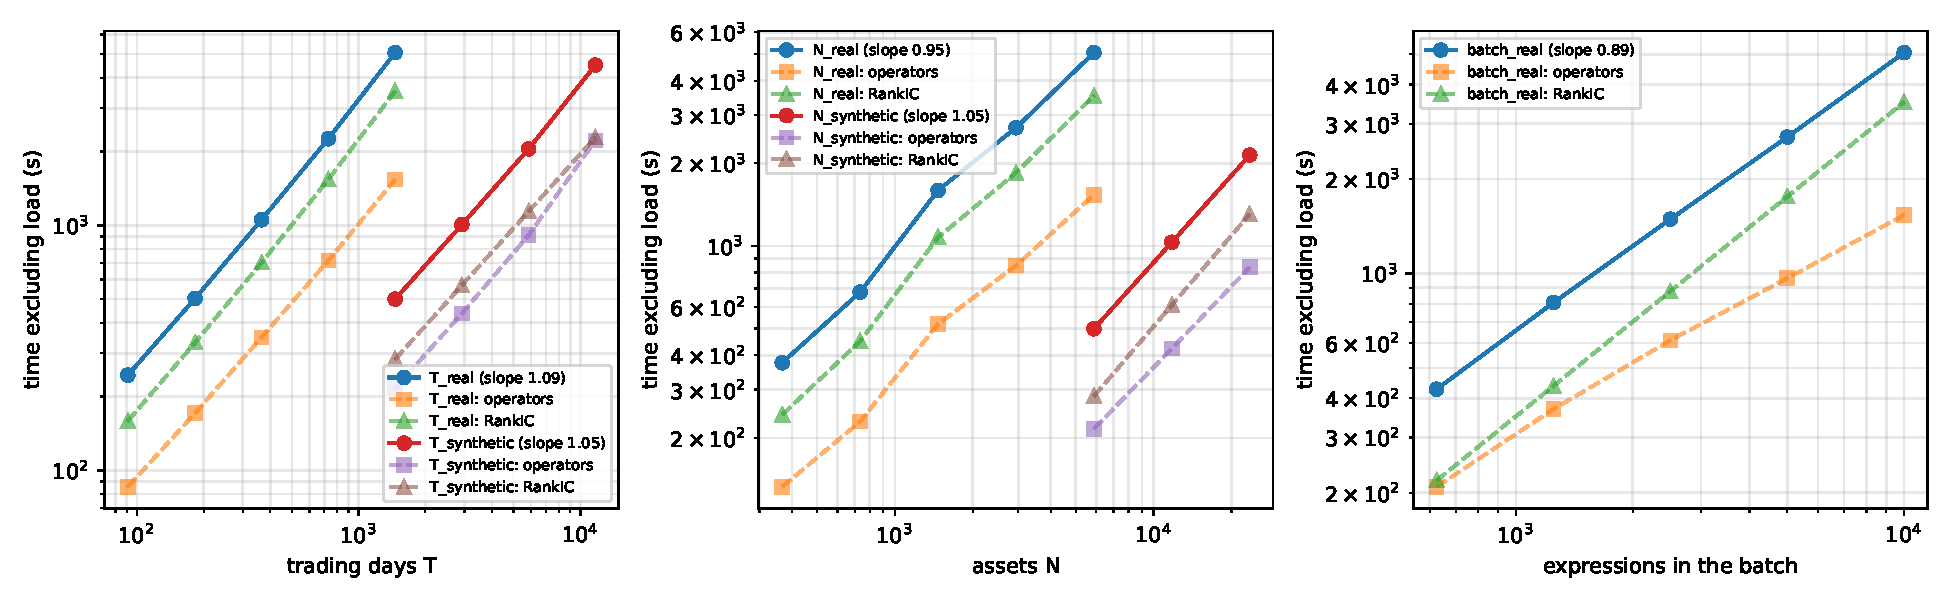
\includegraphics[width=\linewidth]{figures/x1_serial.pdf}
\caption{Serial run time against $T$, $N$ and batch size, with the operator and RankIC parts.}
\label{fig:x1}
\end{figure}

\subsubsection{Strong scaling (pure MPI)}
One thread per rank, $H_0=0$, 1 to 72 ranks on one node and 144 and 288 ranks on two and four nodes.

\begin{table}[h]
\centering
\small
\begin{tabular}{lrrrrrrrrr}
\toprule
ranks & 1 & 2 & 4 & 8 & 16 & 36 & 72 & 144 & 288 \\
nodes & 1 & 1 & 1 & 1 & 1 & 1 & 1 & 2 & 4 \\
\midrule
time (s) & 136.65 & 74.77 & 40.16 & 21.42 & 11.38 & 6.19 & 3.62 & 2.44 & 2.27 \\
speed-up & 1 & 1.83 & 3.40 & 6.38 & 12.0 & 22.1 & 37.8 & 55.9 & 60.2 \\
efficiency & 1 & 0.91 & 0.85 & 0.80 & 0.75 & 0.61 & 0.52 & 0.39 & 0.21 \\
\bottomrule
\end{tabular}
\caption{Strong scaling, 200 factors on the real data.}
\label{tab:x2}
\end{table}

Operators and RankIC keep falling roughly as $1/p$ (at 288 ranks: 1.18\,s and 0.39\,s), but halo exchange plus waiting stays at 1.5--1.9\,s from 16 ranks on (Figure~\ref{fig:x2}). From 144 to 288 ranks the total time barely changes. The Karp--Flatt serial fraction falls from 0.09 at two ranks to about 0.01 and does not grow, so the loss is not a growing serial part but the fixed cost of the level-by-level exchange and of uneven blocks: the dates are split evenly, but later years have more stocks. Per-rank timing to confirm the imbalance is future work.

\begin{figure}[h]
\centering
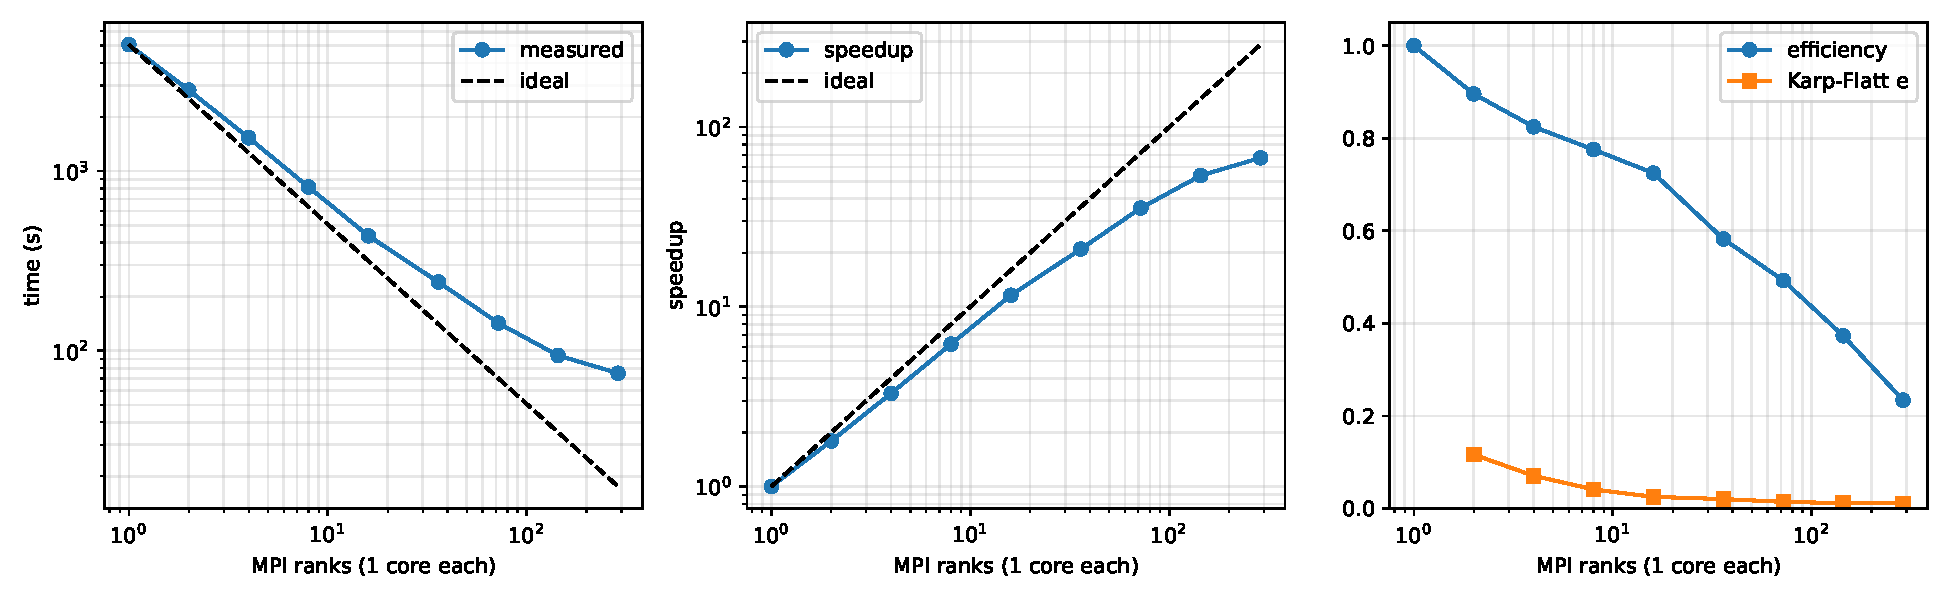
\includegraphics[width=\linewidth]{figures/x2_strong.pdf}
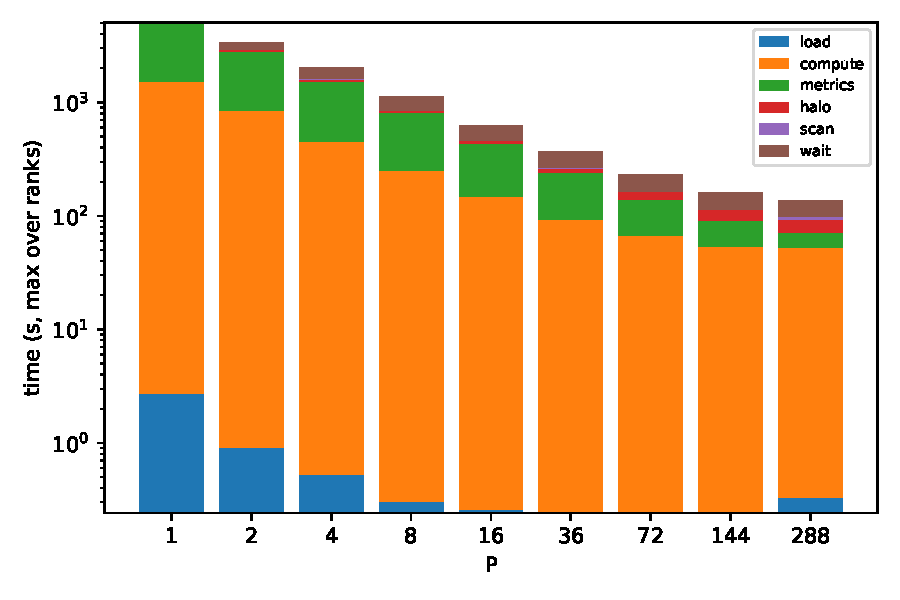
\includegraphics[width=0.6\linewidth]{figures/x2_strong_breakdown.pdf}
\caption{Strong scaling: time, speed-up, efficiency and Karp--Flatt metric (top); time per phase (bottom).}
\label{fig:x2}
\end{figure}

\subsubsection{Weak scaling (pure MPI)}
Synthetic data with 64 days per rank (from $T=64$ at one rank to $T=18432$ at 288 ranks), $N=5876$, 200 factors.

\begin{table}[h]
\centering
\begin{tabular}{lrrrrrr}
\toprule
ranks & 1 & 2--16 & 36 & 72 & 144 & 288 \\
\midrule
time (s) & 9.36 & $\approx$11.0 & 12.69 & 13.19 & 12.97 & 13.60 \\
efficiency & 1 & $\approx$0.85 & 0.74 & 0.71 & 0.72 & 0.69 \\
\bottomrule
\end{tabular}
\caption{Weak scaling on synthetic data.}
\end{table}

The drop from one to two ranks is the halo exchange (about 1.1\,s, then constant). The efficiency falls again between 16 and 72 ranks, when one node is filled and its memory bandwidth is shared, and stays at about 0.7 across two and four nodes, so crossing the network adds little (Figure~\ref{fig:x3}). Synthetic data are used here because the real data cannot grow with the number of ranks; their blocks also have equal work, which separates communication from imbalance.

\begin{figure}[h]
\centering
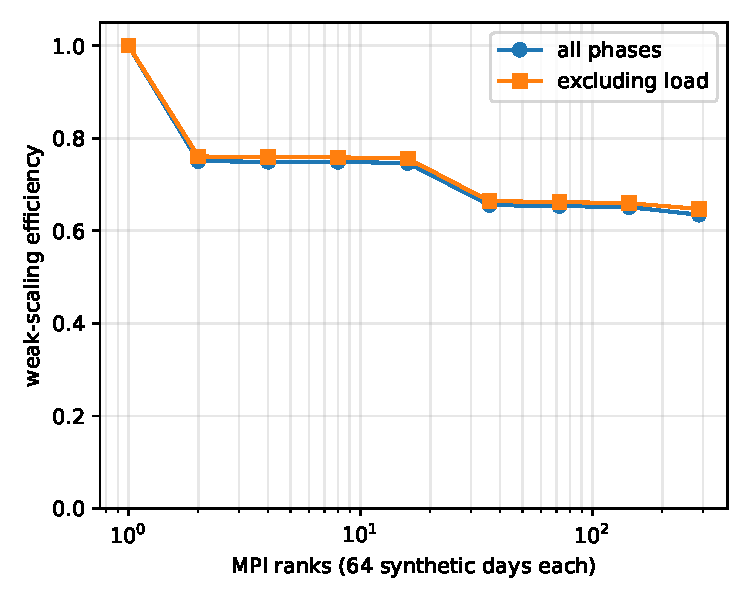
\includegraphics[width=0.45\linewidth]{figures/x3_weak.pdf}
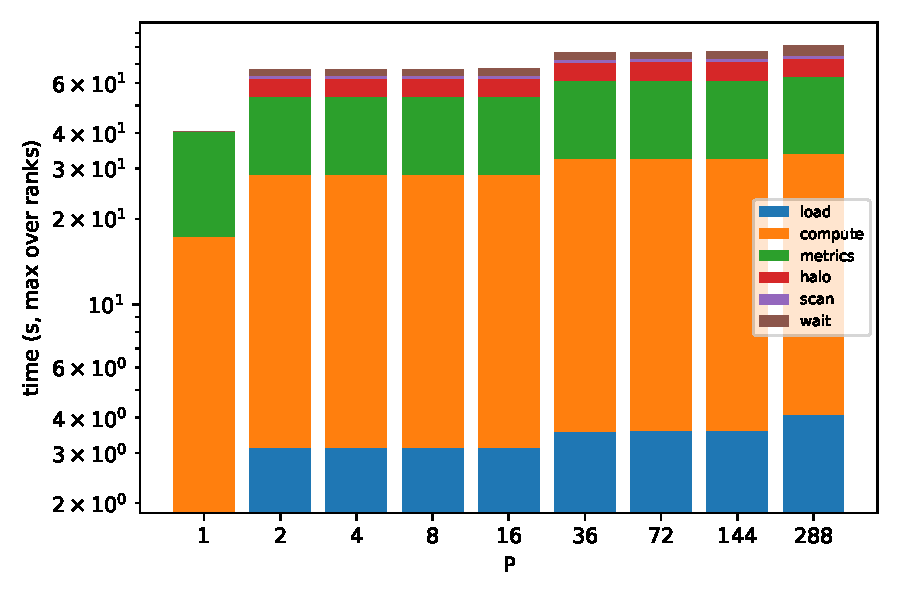
\includegraphics[width=0.5\linewidth]{figures/x3_weak_breakdown.pdf}
\caption{Weak scaling efficiency and time per phase.}
\label{fig:x3}
\end{figure}

\subsubsection{Communication}
\paragraph{Halo exchange versus redundant computation.} With pure MPI, raising $H_0$ from 0 to 89 days cuts the halo data from 7.1--8.0\,MB to 0.7--0.8\,MB and the number of exchanged nodes from 29 to 1, at the cost of 439 redundant rows per rank. The total time changes by less than 2\% at 72, 144 and 288 ranks (Figure~\ref{fig:x4}, left). The halo time is therefore not transfer time: it is time spent waiting for the left neighbour to finish the level. With hybrid splits, $H_0\ge10$ helps 72 ranks $\times$ 4 threads (1.55\,s to 1.38\,s, $-11\%$), does not matter for 16 $\times$ 18, and gives no stable trend for 4 $\times$ 72.

\paragraph{Shared memory versus the network.} The same number of ranks packed on as few nodes as possible or spread over four nodes: 36 ranks take 6.19\,s on one node and 5.44\,s on four; 72 ranks take 3.62\,s and 3.17\,s; 144 ranks take 2.44\,s on two nodes and 2.41\,s on four. Spreading is faster: the extra network hops cost less than sharing one node's memory bandwidth among more ranks.

\paragraph{Which parts communicate most.} Per level each rank sends one packed message to each partner that needs its tail rows; over a batch this is a few megabytes, independent of $p$. The ema chain needs $p-1$ sequential hops but carries only one summary per stock. The fitness needs a single \code{MPI\_Allreduce} of the IC summaries, which takes less than a millisecond. The dominant communication cost is the synchronisation of the halo exchange at every level, not its volume.

\begin{figure}[h]
\centering
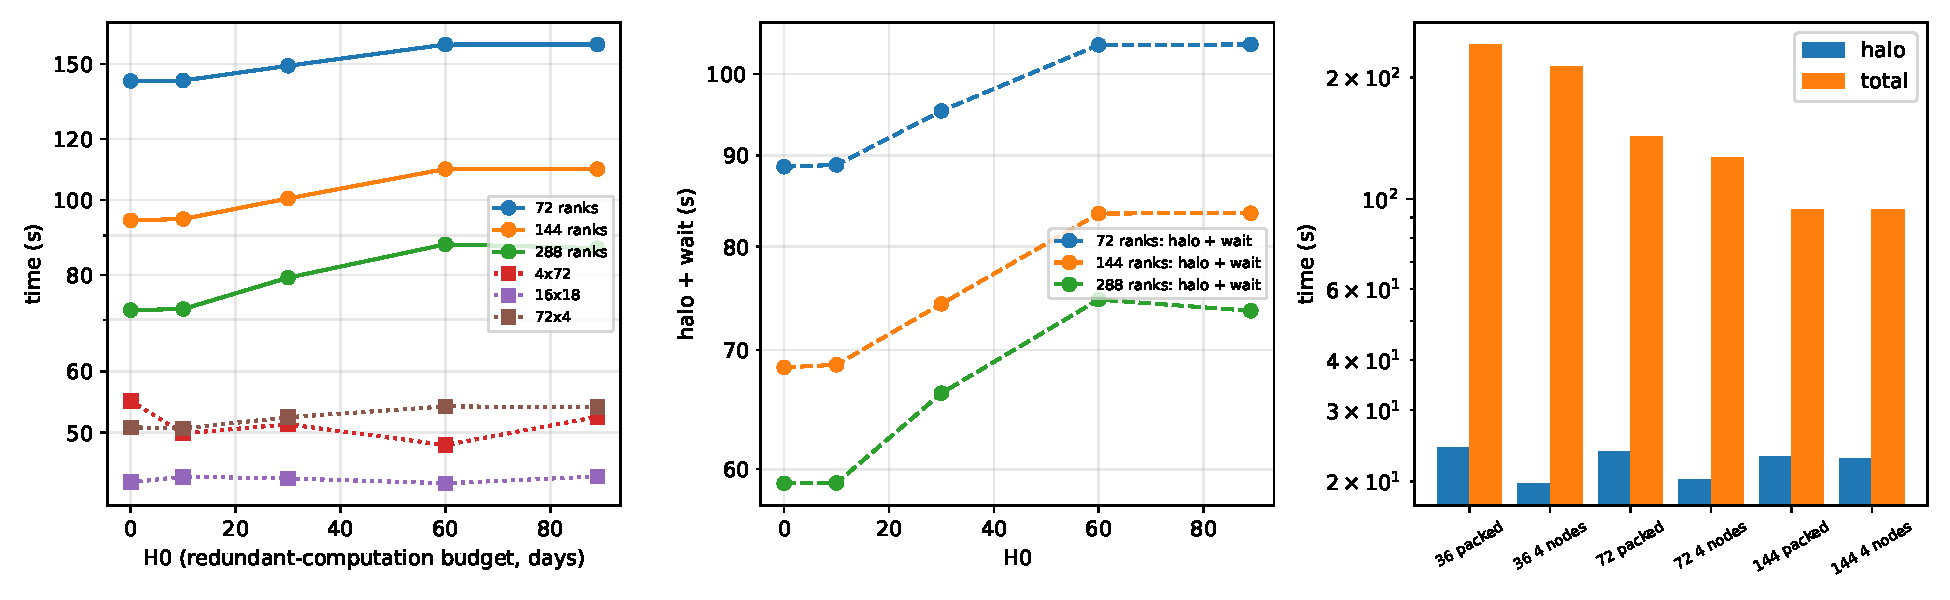
\includegraphics[width=\linewidth]{figures/x4_comm.pdf}
\caption{Left: total time against $H_0$ for pure MPI (solid) and hybrid splits (dotted). Middle: halo plus waiting time. Right: the same rank count packed and spread over four nodes.}
\label{fig:x4}
\end{figure}

\subsubsection{MPI + OpenMP}
\paragraph{One rank.} With one rank and 2 to 72 threads, operator-level threading takes 70.6, 37.5, 19.6, 10.5, 6.13 and 3.82\,s, and node-level threading 68.7, 35.2, 18.4, 10.2, 6.15 and 4.55\,s. Node-level threads are slightly faster up to 16 threads because they avoid opening a parallel region for every operator; at 72 threads they are slower because narrow DAG levels have fewer nodes than threads. On one node, 72 threads (3.82\,s) are as fast as 72 ranks (3.62\,s).

\paragraph{288 cores.} We split four nodes into ranks $\times$ threads (Table~\ref{tab:x5}, Figure~\ref{fig:x5}).

\begin{table}[h]
\centering
\begin{tabular}{lrrrrrrr}
\toprule
ranks $\times$ threads & 288$\times$1 & 144$\times$2 & 72$\times$4 & 36$\times$8 & 16$\times$18 & 8$\times$36 & 4$\times$72 \\
\midrule
operator-level (s) & 2.27 & 1.76 & 1.55 & 1.43 & 1.28 & 1.32 & 1.61 \\
node-level (s) & 2.27 & 1.45 & 1.09 & 1.25 & \textbf{0.98} & 1.06 & 1.44 \\
\bottomrule
\end{tabular}
\caption{288 cores split into MPI ranks and OpenMP threads.}
\label{tab:x5}
\end{table}

The best configuration is 16 ranks $\times$ 18 threads (two ranks per socket) with node-level threads: 0.98\,s, 2.3 times faster than pure MPI on the same 288 cores and 140 times faster than one core. Fewer, larger blocks reduce both the number of exchanging pairs and the imbalance, and the halo time falls from about 0.75\,s to 0.05--0.25\,s. The 36 $\times$ 8 split is slower than its neighbours (1.43\,s and 1.25\,s): nine ranks per node cannot divide two sockets of 36 cores, so OpenMPI cannot bind them, and with the interleaved core numbering of these nodes (even cores on one socket, odd on the other) each rank's threads ended up on both sockets. Within a rank, node-level threading wins on every split, because a rank with a larger block still sees the whole batch DAG and the levels are wide enough to keep the threads busy. Very few ranks (4 $\times$ 72) lose again, probably because each rank spans two sockets and part of its memory traffic crosses between them.

\begin{figure}[h]
\centering
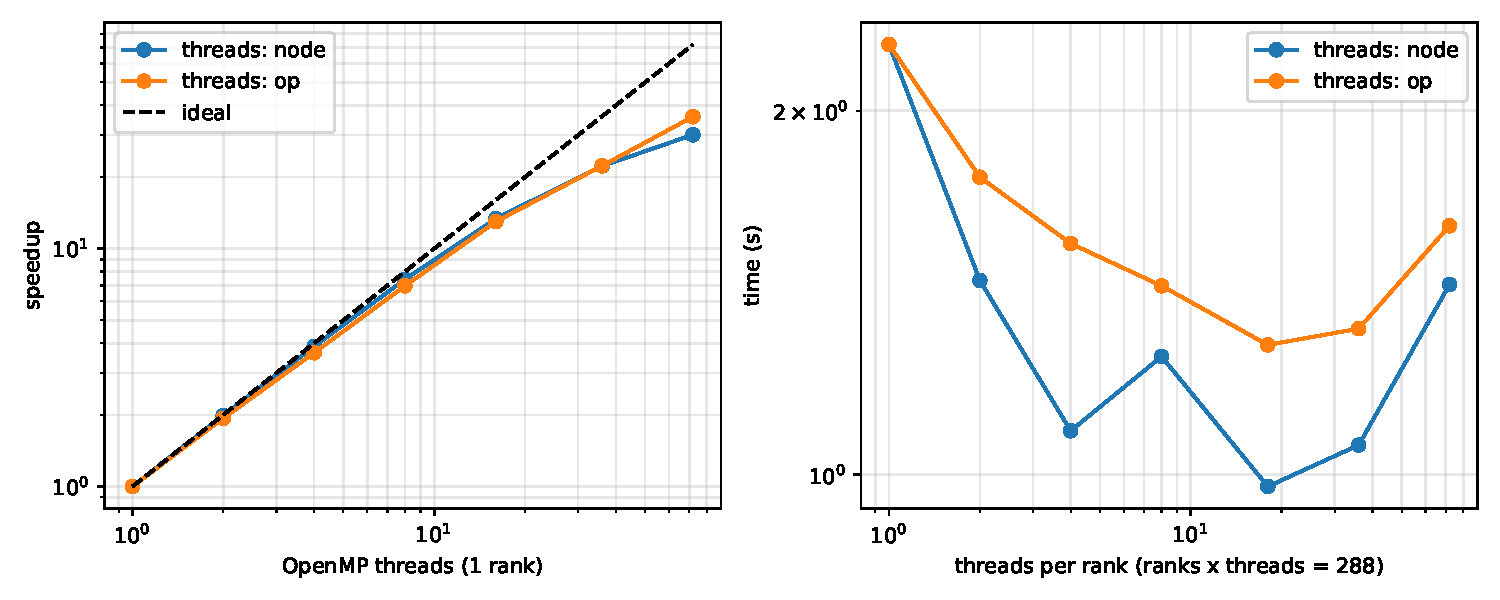
\includegraphics[width=\linewidth]{figures/x5_hybrid.pdf}
\caption{Left: speed-up of one rank with OpenMP threads. Right: 288 cores split into ranks $\times$ threads, with both thread strategies.}
\label{fig:x5}
\end{figure}

\subsubsection{Consistency at scale}
\label{sec:v}
The distributed result is compared with the serial one with the criterion of Section~\ref{sec:validation} (the same candidate validity and $|\Delta\text{fitness}|\le10^{-5}$). It passes for 16 ranks, 4 ranks $\times$ 4 threads with both thread strategies, 4 ranks with $H_0=30$, 72 ranks on one node, 288 ranks on four nodes, and 16 ranks $\times$ 18 threads with node-level threads on four nodes.

\subsection{PCA signatures and similarity}

\subsubsection{Serial cost}
\todo{}

\subsubsection{GPU kernels against the CPU}
\todo{}

\subsubsection{MPI + CUDA scaling}
\todo{}

\subsubsection{Agreement of signatures and admission decisions}
\todo{}

\subsection{Power iteration versus Lanczos}

\subsubsection{Accuracy against iterations}
\todo{}

\subsubsection{Cost}
\todo{}

\subsubsection{Effect on admission decisions}
\todo{}

\subsection{DAG, memory and caching}

\subsubsection{Subexpression sharing}
\todo{}

\subsubsection{Peak memory against batch size}
\todo{}

\subsubsection{Reuse across generations}
\todo{}

\subsubsection{Cache policies}
\todo{}

%======================================================================
\section{Discussion}

\subsection{How each part is parallelised}
\todo{table: module $\times$ technique (MPI, OpenMP, CUDA) $\times$ communication volume $\times$ bottleneck; which part needs the most communication}

\subsection{Conclusions about the data}
\todo{growing stock universe and load imbalance; distribution of RankIC of the selected factors; effect of float32 on rankings}

\subsection{Future work}
\todo{asynchronous steady-state GP; overlapping CPU and GPU work; evaluating immigrants early instead of waiting for the generation's PCA step; \code{MPI\_Exscan} for ema; weighted date blocks; fusion of element-wise operators}

%======================================================================
\section{Conclusion}
\todo{}

\section*{Use of AI tools}
\todo{Describe honestly how AI assistants were used, for example design discussion, code drafting and review, and how the results were verified.}

\appendix
\section{Code structure, building and running}
\todo{directory layout}
\begin{lstlisting}
module load OpenMPI/5.0.8-GCC-14.3.0 CMake/4.0.3-GCCcore-14.3.0
cmake -S . -B build_vanda -DGPE_ENABLE_MPI=ON
cmake --build build_vanda -j
qsub scripts/vanda/build_test.pbs      # build and validation tests
bash scripts/vanda/submit.sh           # experiment jobs
python python/scripts/plot_vanda.py <csv_dir> <figure_dir>
\end{lstlisting}

\end{document}
